\documentclass[12pt,letter]{article}
\usepackage{mathptmx} % added for time new roman font
\usepackage[left=1in,right=1in,top=1in,bottom=1in]{geometry}
\usepackage[latin1]{inputenc}
\usepackage{amsmath}
\usepackage[final]{pdfpages}

\usepackage[textsize=tiny]{todonotes}

% defines all example enviorment
\usepackage[framemethod=tikz]{mdframed} % added for the box around examples
\newtheorem{ex}{Example}
\numberwithin{ex}{section} % allows for the use of example numbers that lign up with the section numbers
\newenvironment{example}{\begin{mdframed}[middlelinewidth=0.5mm]\begin{ex}\normalfont}{\end{ex}\end{mdframed}}

% defines all review enviorment
\usepackage[framemethod=tikz]{mdframed} % added for the box around examples
\newtheorem{re}{Review}
\numberwithin{re}{section} % allows for the use of example numbers that lign up with the section numbers
\newenvironment{review}{\begin{mdframed}[middlelinewidth=2mm,roundcorner=20pt]\begin{re}\normalfont}{\end{re}\end{mdframed}}

% defines the quotation enviorment 
\usepackage{xcolor}
\newcommand{\quotebox}[2]{\begin{center}\fcolorbox{white}{blue!15!gray!15}{\begin{minipage}{0.9\linewidth}\vspace{10pt}\center\begin{minipage}{0.8\linewidth}{\space\Huge``}{#1}{\Huge''}{\break\null\hfill} {\small #2}  \end{minipage}\medbreak\end{minipage}}\end{center}}

% defines the definition enviorment 
\newcommand{\definitionbox}[2]{\begin{center}\fcolorbox{white}{blue!15!gray!15}{\begin{minipage}{0.9\linewidth}\vspace{10pt}\center\begin{minipage}{0.8\linewidth} {{\textbf{Definition} - }{#1}: {#2}}\end{minipage}\medbreak\end{minipage}}\end{center}}

\usepackage{amsfonts}
\usepackage{amssymb}
\usepackage{graphicx}
\usepackage{float}
\usepackage{booktabs}
%\usepackage{parskip} % remove all the paragraph indents
\usepackage{xfrac}
\usepackage{upgreek}
\usepackage{wrapfig}
\usepackage{setspace}
\usepackage[colorlinks=true]{hyperref}
\usepackage{textcomp} 
\usepackage{multicol} 
\usepackage{enumitem}		% added for spacing in itemize lists
\usepackage[numbered,framed]{matlab-prettifier}		% added for matlab code
\let\ph\mlplaceholder % shorter macro
\lstMakeShortInline"
\lstset{
  style              = Matlab-editor,
  basicstyle         = \mlttfamily,
  escapechar         = ",
  mlshowsectionrules = true,
}

\usepackage{color} % color added for editing
\newcommand{\bl}[1]{\textcolor[rgb]{0.00,0.00,1.00}{#1}}
\newcommand{\gr}[1]{\textcolor[rgb]{0.00,0.50,0.00}{#1}}
\newcommand{\rd}[1]{\textcolor[rgb]{0.75,0.00,0.00}{#1}}

\usepackage{fancyhdr}
\pagestyle{fancy}
\fancyfoot{} % clear all footer fields
\fancyfoot[LE,RO]{Page \thepage} 
\fancyfoot[RE,LO]{}

%%%%%%%		define the symbols for positive directions		%%%%%%
\makeatletter													%%	
																%%					
\newcommand*\curveplus{% positive counterclockwise				%%
  \mathbin{\rotatebox[origin=c]{90}{$\m@th\curvearrowleft$}+}}	%%
																%%
\newcommand*\rightplus{% positive right							%%
  \mathpalette\@rightplus\relax}								%%
\newcommand*\@rightplus[1]{%									%%
  \mathbin{\vcenter{\hbox{$\m@th\overset{#1+}{\to}$}}}}			%%
																%%	
\newcommand*\upplus{% positive up								%%
  \mathbin{+\mathord\uparrow}}									%%
																%%			
\newcommand*\downplus{% positive down							%%		
  \mathbin{+\mathord\downarrow}}								%%
  																%%		
\newcommand*\downrightplus{% positive down and right			%%	
  \mathbin{+ \rotatebox[origin=c]{-30}{$\m@th\rightarrow$}}}	%%
\makeatother 													%%	
%%%%%%%%%%%%%%%%%%%%%%%%%%%%%%%%%%%%%%%%%%%%%%%%%%%%%%%%%%%%%%%%%%


\usepackage{mathtools}          %loads amsmath as well added for the piece wise function
\DeclarePairedDelimiter\Floor\lfloor\rfloor
\DeclarePairedDelimiter\Ceil\lceil\rceil

 
\newcounter{NumberInTable}
\newcommand{\LTNUM}{\stepcounter{NumberInTable}{(\theNumberInTable)}}

\newcommand{\Laplace}[1]{\ensuremath{\mathcal{L}{\left[#1\right]}}}
\newcommand{\InvLap}[1]{\ensuremath{\mathcal{L}^{-1}{\left[#1\right]}}}
\renewcommand{\textuparrow}{$\uparrow$}

\numberwithin{equation}{section}	% added so the equsation numbers are section.# and start at section.1

\begin{document}
%	
%	\large{}
%	
%	\title{\vspace{-2cm} Chapter 1: Basic concepts of Control Theory}
%	\date{}
%	\maketitle

	% set the section number, along with figure and equation numbers
	\setcounter{section}{3}	
	\setcounter{figure}{0}   
	\renewcommand\thefigure{\thesection.\arabic{figure}}


\section{Time Series Response}

\subsection{Transfer Functions Block Diagrams}


Transfer functions can be created using:

\begin{itemize}[noitemsep,topsep=0pt]
	\item Polynomial model (numerator / denominator)
\end{itemize}
\begin{equation}
	G(s) = \frac{B(s)}{A(s)} = \frac{b_ms^m + b_{m-1}s^{m-1} + ... + b_0}{a_ns^n + a_{n-1}s^{n-1} + ... + a_0}
\end{equation}
\begin{itemize}[noitemsep,topsep=0pt]
\item[]
	\begin{itemize}[noitemsep,topsep=0pt]
		\item $n$ = order of transfer function models where $m <n$
	\end{itemize}
	\item Zero-pole-gain model (numerator / denominator)
\end{itemize}
\begin{equation}
	G(s) = k \frac{(s-z_1)(s-z_2)\cdots (s-z_m)}{(s-p_1)(s-p_2)\cdots (s-p_n)}
\end{equation}
\begin{itemize}[noitemsep,topsep=0pt]
\item[]
\begin{itemize}[noitemsep,topsep=0pt]
	\item zeros: $z_1$, $z_2, \cdots, z_m$ roots of $B(s)=0$ 
	\item poles: $p_1$, $p_2, \cdots, p_n$ roots of $A(s)=0$ 
	\item gain: $k$
\end{itemize}
\item Time constant model
\end{itemize}
 \begin{equation}
G(s) = \frac{k}{s^N} \cdot \frac{(T_a + 1)(T_b + 1)\cdots}{(T_1 + 1)(T_2 + 1)\cdots}
\end{equation}
\begin{itemize}[noitemsep,topsep=0pt]
\item[] \begin{itemize}[noitemsep,topsep=0pt]
\item $N$ = type of transfer function model
\end{itemize}
\end{itemize}

\subsubsection{Create transfer function using numerator and denominator coefficients}


MATLAB can be used to create continuous-time single-input, single-output (SISO) transfer functions from their numerator and denominator coefficients using \texttt{tf}. To use the tf function, you must have the Control System Toolbox licensed and installed. To find out if you do, type: \texttt{ver control} in your Command Window or a script. \\

\noindent \textbf{Method I}

Create the transfer function 
\begin{equation}
G(s) = \frac{s}{s^2 + 3s + 2}
\end{equation}


\lstset{linewidth=5.8in}
\begin{minipage}{1\textwidth}
  \begin{center}
    \lstset{%
caption={MATLAB code for Method I.},
      basicstyle=\ttfamily\footnotesize\bfseries,
      frame=tb,
    }
\begin{lstlisting}
num = [1 0];
dem = [1 3 2];
G = tf(num, dem) 
% To use the tf function, you must have the Control System Toolbox
% licensed and installed. To find out if you do, type: 
% "ver control" in your Command Window or a script.  
\end{lstlisting}
  \end{center}
\end{minipage}
where \texttt{nem} and \texttt{dem} are the numerator and denominator polynomial coefficients in descending powers of $s$. For example, \texttt{den = [1 3 2]} represents the denominator polynomial $\frac{s}{s^2 + 3s + 2}$

\texttt{G} is a \texttt{tf} model object, which is a data container for representing the transfer function in polynomial form. \\


\noindent \textbf{Method II}

Alternatively, you can specify the transfer function $G(s)$ as an expression in $s$-domain.
\begin{enumerate}[noitemsep,topsep=0pt]
\item Create a transfer Function model for the variable $s$
\item Specify $G(s)$ as a ratio of polynomials in $s$
\end{enumerate}

\lstset{linewidth=5.8in}
\begin{minipage}{1\textwidth}
  \begin{center}
    \lstset{%
caption={MATLAB code for Method II.},
      basicstyle=\ttfamily\footnotesize\bfseries,
      frame=tb,
    }
\begin{lstlisting}
s = tf('s');
G = s/(s^2+3*s+2)
\end{lstlisting}
  \end{center}
\end{minipage}

Therefore, the full expression of $G(s)$ can be written as
\begin{equation}
G(s) = \frac{B(s)}{A(s)} = \frac{s}{s^2 + 3s + 2} = \frac{b_1s + b_0}{a_1s^2 + a_2 s + a_0}
\end{equation}
where 
\begin{equation}
B(s) = b_1s + b_0 
\end{equation}
resulting in  $b_1=1$, and $b_0=0$; or, \texttt{B = [1 0]}. Moreover, 
\begin{equation}
A(s) = a_1s^2 + a_2 s + a_0
\end{equation}
where $a_1=1$, $a_1=3$, and $a_0=1$; or, \texttt{A = [1 3 1]}.

\subsubsection{Create transfer function using Zeros, Poles, and Gain}

MATLAB can be used to create continuous-time single-input, single-output (SISO) transfer functions in factored form using \texttt{zpk}. Create the factored transfer function 
\begin{equation}
G(s) =  5 \frac{s}{(s-1-i)(s-1-i)(s-2)}
\end{equation}

\lstset{linewidth=5.8in}
\begin{minipage}{1\textwidth}
  \begin{center}
    \lstset{%
caption={MATLAB code to create a transfer function using Zeros, Poles, and Gain.},
      basicstyle=\ttfamily\footnotesize\bfseries,
      frame=tb,
    }
\begin{lstlisting}
Z = 0;
P = [-1-1i -1+1i -2]; 
K = 5;
G = zpk(Z,P,K)
\end{lstlisting}
  \end{center}
\end{minipage}

\noindent where \texttt{Z} and \texttt{P} are zeros and poles (the roots of the numerator and denominator respectively). K is the gain of the factored from. Solving fore the poles $p_1$, $p_2$, and $p_3$ of $G(s)$;
\begin{align}
G(s) &=  5 \frac{s}{(s-1-i)(s-1-i)(s-2)} \\
&=  5 \frac{s-0}{\big[s-(-1-i)\big]\big[(s-(-1-i)\big]\big[(s-(-2)\big]} \nonumber \\
\end{align}
where $K=5$, $s-0=s-z_1 \rightarrow z_1 = 0$, and $Z=[0]$. Therefore, 
\begin{equation}
\big[s-(-1-i)\big]\big[(s-(-1-i)\big]\big[(s-(-2)\big] = (s-p_1)(s-p_2)(s-p_3)
\end{equation}
this leads to
\begin{equation}
G(s) =  k \frac{s-z_1}{(s-p_1)(s-p_2)(s-p_3)}
\end{equation}
therefore, $G(s)$ has a real pole at $s=-2$ and a pair of complex poles as $s= -1 \pm i$. The vector \texttt{P = [-1-1i -1+1i -2]} specifies these pole locations.

\subsection{Order verse Type}

\todo{need to find some real-world examples of orders and types.}

A system has a ``Type'' and an ``Order'', which have different meanings. 
\begin{itemize}[noitemsep,topsep=0pt]
\item Order = $n$, highest exponent of $s$ in the denominator. $n$ is the number of poles.
\item Type = $N$, exponent of the factored out $s$ in the denominator. $N$ is the number of poles in origin ($p=0$). 
\end{itemize}

Consider the 1\textsuperscript{st}-order mass-damper system (no stiffness) as shown in figure \rd{X} with the transfer function

\todo{make a figure}

\begin{equation}
G(s) = \frac{\omega_n^2}{s^2 + 2 \zeta \omega_n s} 
\end{equation}
The transfer function can easily be written in the basic form 
\begin{equation}
G(s) = \frac{b_0}{a_2s^2+a_1s}
\end{equation}
where $a_2=1$, $a_1=2 \zeta \omega_n$, $b_0 = \omega_n^2$. There the presence of $a_2$ means its a 2\textsuperscript{nd} order system. To solve for the type of the system, $s$ must be factored of of the denominator, leading to:

\begin{align}
G(s) &= \frac{\omega_n^2}{s^2 + 2 \zeta \omega_n s} \\
&= \frac{\omega_n^2}{s(s+2 \zeta \omega_n)} \nonumber \\
&= \frac{\frac{\omega_n}{2 \zeta}}{s} \cdot \frac{1}{\frac{1}{2 \zeta \omega_n}s+1} \nonumber \\
&= \frac{K}{s^N} \cdot \frac{1}{T_1s+1} \nonumber
\end{align}
where $K=\frac{\omega_n}{2 \zeta}$, $N=1$, and $T_1 = \frac{1}{2 \zeta \omega_n}$. $N=1$ means that is a Type 1 system. Therefore, this is a 2\textsuperscript{nd} order system of Type 1, ``Type'' and ``Order'' have different meanings. Table~\ref{table:types_and_orders} reports the types and orders for different transfer functions.

\begin{table}[H]
\centering
\label{table:types_and_orders}
\caption{Examples of types and orders for different transfer functions.}
\begin{tabular}{@{}lll@{}}
\toprule
transfer function & Type & Order \\ \midrule
 $G(s) = \frac{1}{Ts+1}$& 0 & 1 \\
 $G(s) = \frac{1}{cs} =    \frac{\sfrac{1}{c}}{s} $  & 1 & 1 \\
  $G(s) = \frac{1}{Js^2} = \frac{\sfrac{1}{J}}{s^2}$ & 2 & 2 \\
 $G(s) = \frac{1}{Js^2 + cs} = \frac{K/c}{s} \cdot \frac{1}{\sfrac{J}{c}s+1}$ & 1 & 2 \\
 \parbox{3cm}{\begin{align}
    G(s) &= \frac{K}{J^4} \frac{T_a s + 1}{(T_1s+1)(T_2s+1)(T_3s+1)} \nonumber \\
     &= \frac{b_1 s + b_0}{s^4 (a_3 s^3 + a_2 s^2 + a_1 s + a_0) } \nonumber \\
 	&= \frac{b_1 s + b_0}{(a_3 s^7 + a_2 s^6 + a_1 s^5 + a_0s^4) } \nonumber
  \end{align}}& 4 & 7 \\ \bottomrule
\end{tabular}
\end{table}
\subsection{Time Response}


Time response calculations are obtained using the Laplace transforms where the Laplace transform is
\begin{equation}
X(s) = G(s)F(s)
\end{equation}
and the time response is 
\begin{equation}
x(t) = \Laplace{X(s)}^{-1}
\end{equation}

\subsubsection{Time Series Response for a Step Function}

		\begin{figure}[H]
			\centering
			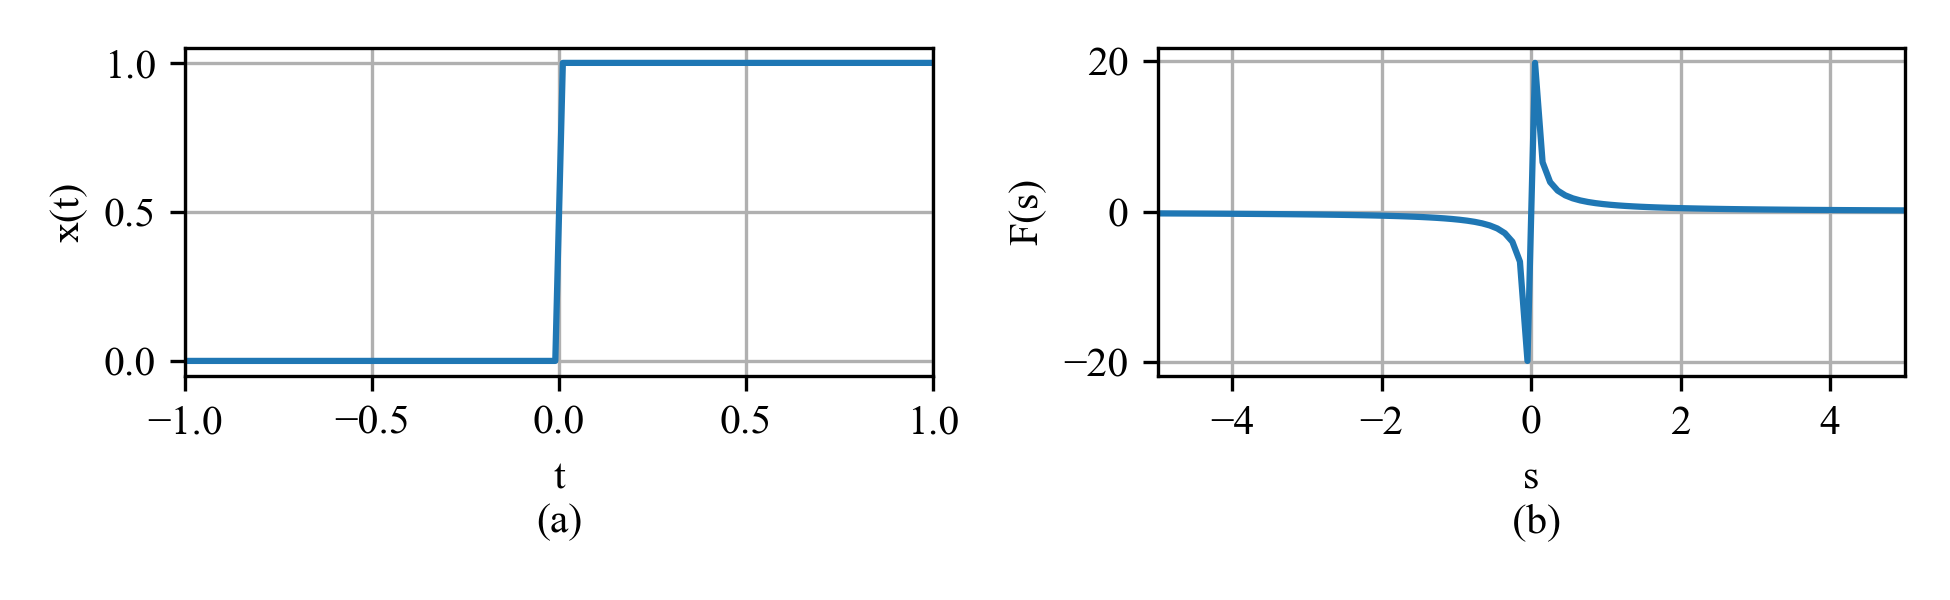
\includegraphics[width=6.5in]{../figures/T_and_S_space_step_function}
			\caption{Step function; showing the (a) time domain and; (c) the s-space.}
			\label{fig:T_and_S_space_step_function}
		\end{figure}


A step function is expressed as the following Laplace pair:
		\begin{equation}
		\text{LT pair} =
			\begin{cases}
			f(t) & 1(t) , \; \; \; t>0 \\
			F(s) & \frac{1}{s} \\
			\end{cases}
		\end{equation}
therefore, the time response of the systems is expressed as
\begin{equation}
x(t) = \Laplace{G(s) \frac{1}{s}}^{-1}
\end{equation}
In MATLAB, this is expressed as:

\lstset{linewidth=5.8in}
\begin{minipage}{1\textwidth}
  \begin{center}
    \lstset{%
caption={MATLAB code for the time-series resposne of a step function.},
      basicstyle=\ttfamily\footnotesize\bfseries,
      frame=tb,
    }
\begin{lstlisting}
x_t = step(G)
\end{lstlisting}
  \end{center}
\end{minipage}

\subsubsection{Time Series Response for a Impulse Function}



		\begin{figure}[H]
			\centering
			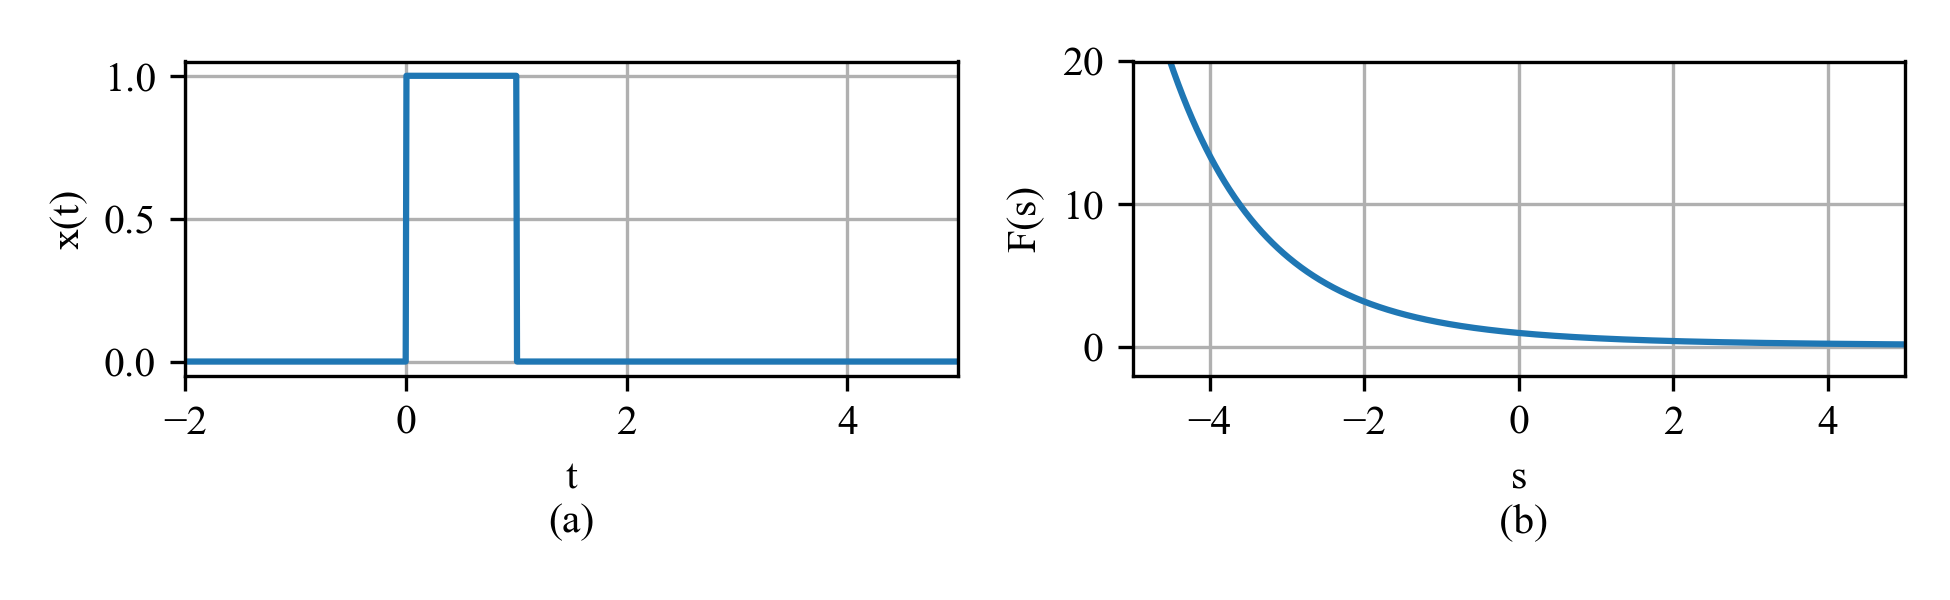
\includegraphics[width=6.5in]{../figures/T_and_S_pulse_function}
			\caption{Pulse function; showing the (a) time domain and; (c) the s-space.}
			\label{fig:Laplace_pulse_transform}
		\end{figure}


An impulse function is expressed as the following Laplace pair:
		\begin{equation}
		\text{LT pair} =
			\begin{cases}
			f(t) & p(t; \; \; \tau) \\
			F(s) & \frac{1-e^{-st\tau}}{s \tau}
			\end{cases}
		\end{equation}
therefore, the time response of the systems is expressed as
\begin{equation}
x(t) = \Laplace{G(s) \frac{1-e^{-st\tau}}{s \tau}}^{-1}
\end{equation}
In MATLAB, this is expressed as:

\lstset{linewidth=5.8in}
\begin{minipage}{1\textwidth}
  \begin{center}
    \lstset{%
caption={MATLAB code for the time-series resposne of a step function.},
      basicstyle=\ttfamily\footnotesize\bfseries,
      frame=tb,
    }
\begin{lstlisting}
x_t = impulse(G)
\end{lstlisting}
  \end{center}
\end{minipage}


\subsubsection{Time Series Response for a Ramp Function}



		\begin{figure}[H]
			\centering
			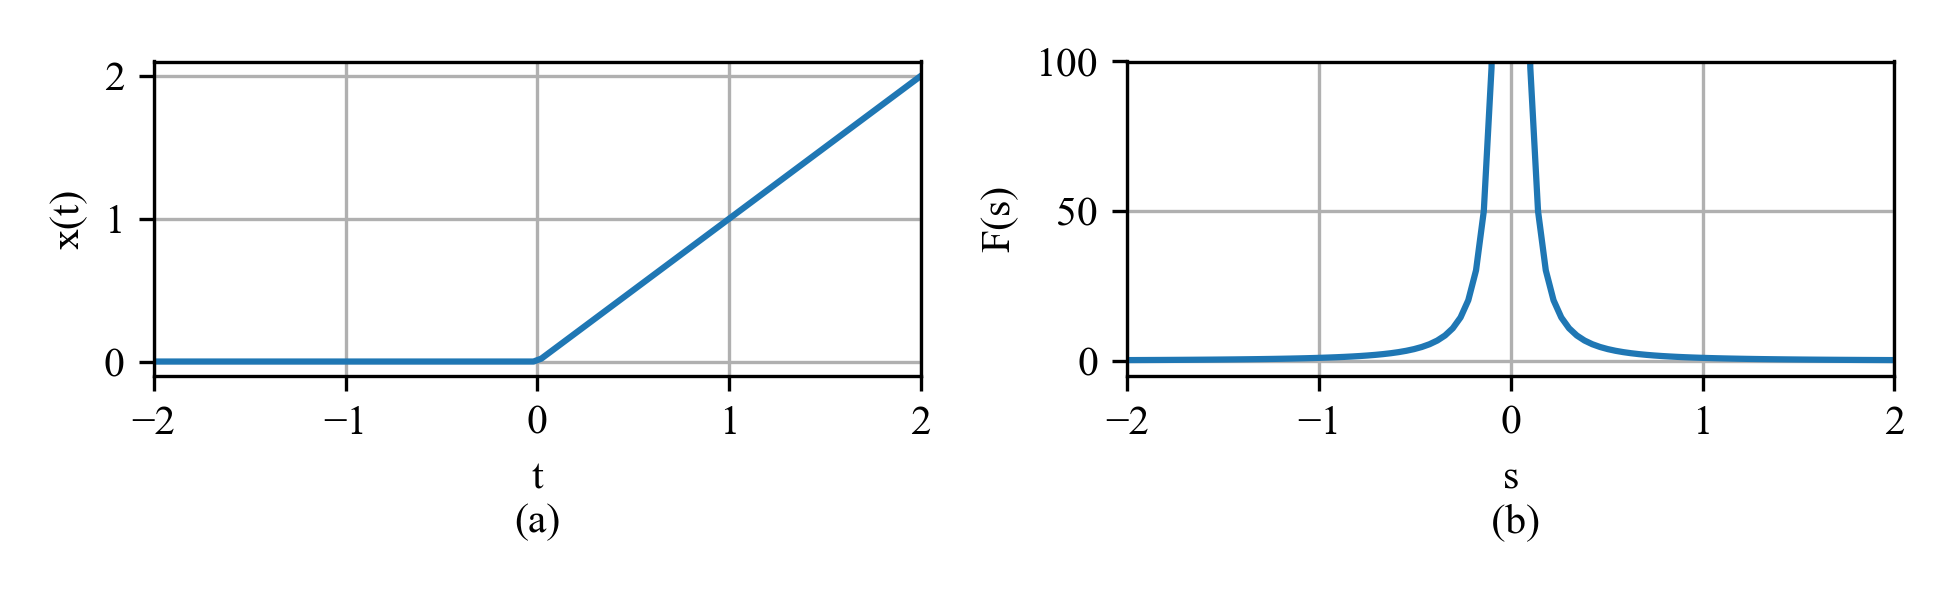
\includegraphics[width=6.5in]{../figures/T_and_S_space_ramp_function}
			\caption{Ramp function; showing the (a) time domain and; (c) the s-space.}
			\label{fig:T_and_S_space_ramp_function}
		\end{figure}

An ramp function is expressed as the following Laplace pair:
		\begin{equation}
		\text{LT pair} =
			\begin{cases}
			f(t) & t, \; \; \; t>0 \\
			F(s) & \frac{1}{s^2} \\
			\end{cases}
		\end{equation}
therefore, the time response of the systems is expressed as
\begin{equation}
x(t) = \Laplace{G(s) \frac{1}{s^2}}^{-1}
\end{equation}
In MATLAB, this is expressed as:

\lstset{linewidth=5.8in}
\begin{minipage}{1\textwidth}
  \begin{center}
    \lstset{%
caption={MATLAB code for the time-series resposne of a step function.},
      basicstyle=\ttfamily\footnotesize\bfseries,
      frame=tb,
    }
\begin{lstlisting}
x_t = impulse(G/(s^2))
\end{lstlisting}
  \end{center}
\end{minipage}

Note that for the MATLAB code, we used the property:
\begin{equation}
X(s) = G(s) \frac{1}{s^2} = \Big(\frac{G(s)}{s^2}\Big) \cdot 1
\end{equation}
where 1 is the Laplace transform of an impulse. Note that \texttt{ramp} is not an option in MATLAB as this command is already used to generate a time-series ramp signal. 


\subsection{1\textsuperscript{st} Order System Time Response}

The first order equation of motion is
\begin{equation}
T \dot{x}(t) + x(t) = f(t)
\end{equation}
where $x(0)=0$ is the initial condition and $T$ is a time constant for the first order system. The Laplace transform gives us
\begin{align}
x & \rightarrow X(s) \\
\dot{x} & \rightarrow sX(s) \nonumber \\
f(t) & \rightarrow F(s) \nonumber 
\end{align}
therefore, the s-domain equation is:
\begin{equation}
TsX(s) + X(s) = F(s)
\end{equation}
where:
\begin{equation}
X(s) = \frac{F(s)}{T s + 1} = \frac{1}{Ts + 1}F(s) = G(s)F(s)
\end{equation}
therefore, the transfer function is:
\begin{equation}
G(s) = \frac{1}{T s + 1}
\end{equation}

\begin{figure}[H]
	\centering
	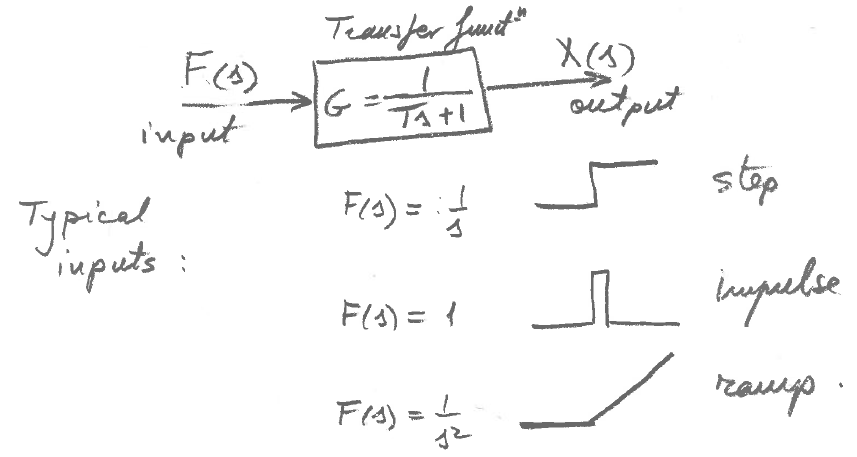
\includegraphics[width=5.5in]{../figures/time_response_1st_order}
\end{figure}

\subsubsection{Step response of a 1\textsuperscript{st} Order System}

\begin{align}
X(s) &= G(s)F(s) \\
&= \frac{1}{Ts+1} \cdot \frac{1}{s} \nonumber \\
&= \frac{1}{s(Ts+1)}
\end{align}
Therefore, solving for $\Laplace{X(s)}^{-1}$ yields
\begin{equation}
x(t) = 1-e^{-t/T}
\end{equation}
or
\begin{figure}[H]
	\centering
	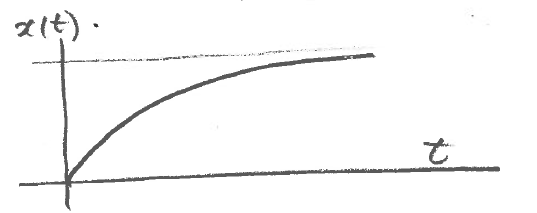
\includegraphics[width=3.5in]{../figures/x_t_time_response}
\end{figure}


\subsubsection{Impulse response of a 1\textsuperscript{st} Order System}


\begin{align}
X(s) &= G(s)F(s) \\
&= \frac{1}{Ts+1} \cdot 1 \nonumber \\
&= \frac{1}{Ts+1}
\end{align}
Therefore, solving for $\Laplace{X(s)}^{-1}$ yields
\begin{equation}
x(t) = \frac{1}{T}e^{-t/T}
\end{equation}
or
\begin{figure}[H]
	\centering
	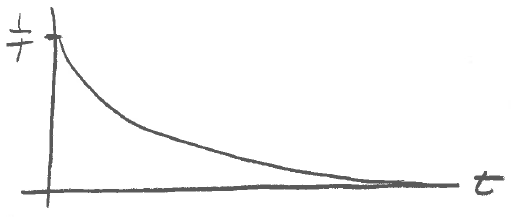
\includegraphics[width=3.5in]{../figures/x_t_impulse_time_response}
\end{figure}


\subsubsection{Ramp response of a 1\textsuperscript{st} Order System}


\begin{align}
X(s) &= G(s)F(s) \\
&= \frac{1}{Ts+1} \cdot \frac{1}{s^2} \nonumber \\
&= \frac{1}{s^2(Ts+1)}
\end{align}
Therefore, solving for $\Laplace{X(s)}^{-1}$ yields
\begin{align}
x(t) &= t - T + Te^{-t/T} \nonumber \\
&= t - T\big(1-e^{-t/T}\big)
\end{align}
or
\begin{figure}[H]
	\centering
	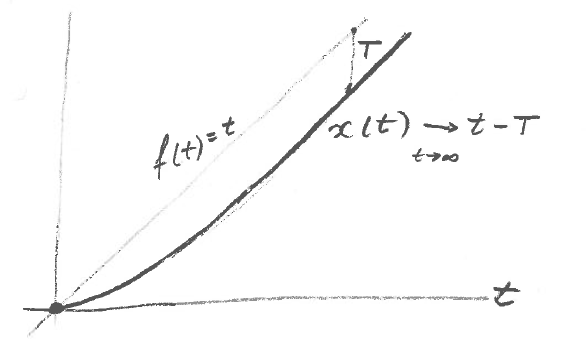
\includegraphics[width=3.5in]{../figures/x_t_ramp_time_response}
\end{figure}
Moreover, 
\begin{equation}
x(t) = t-T+Te^{-t/T}  \xrightarrow[t \rightarrow \infty]{} t-T
\end{equation}

\subsubsection{Summary of the First Order System Responses}

\begin{figure}[H]
	\centering
	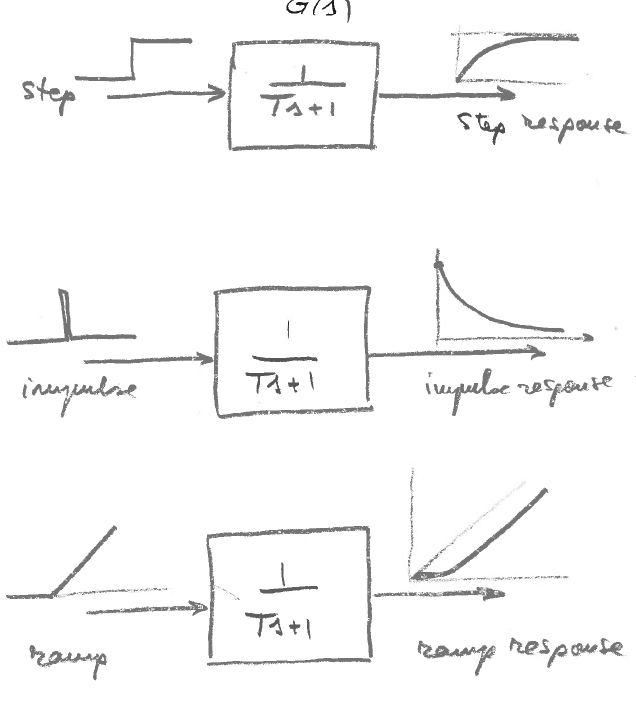
\includegraphics[width=4.5in]{../figures/Summary_of_first_order_system_response}
	\caption{A summary of the first order system responses.}
\end{figure}


\lstset{linewidth=5.8in}
\begin{minipage}{1\textwidth}
  \begin{center}
    \lstset{%
caption={MATLAB code for time series responses of 1\textsuperscript{st} order system.},
      basicstyle=\ttfamily\footnotesize\bfseries,
      frame=tb,
    }
\begin{lstlisting}
%{
This program studies time response of 1st order systems
%}
clc
clear
close all

format compact

%% Given data
T=2.5; % time response for the 1D system

%% time range setup
T_max = 10;         % run the test to 10 seconds
dt = T_max*1e-4;    % find the delta-t value 
t = 0:dt:T_max;     % build the time vector

%% Define system
B = [1];
A = [T 1];
G = tf(B,A); 

%% create the figure enviorment
figure(1)

%% step response 
subplot(3,1,1)
hold on
step(G,t)
ylim([0 1.2])

%% Impulse response
subplot(3,1,2)
impulse(G,t)

%% Ramp response
F_ramp = tf([1],[1 0 0])
subplot(3,1,3)
impulse(G*F_ramp,t)
title('Ramp Response') % need to set manually. 
\end{lstlisting}
  \end{center}
\end{minipage}


\begin{figure}[H]
	\centering
	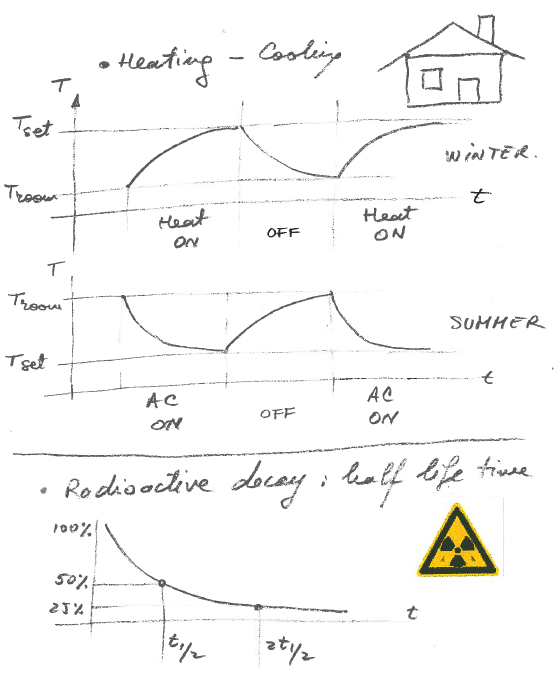
\includegraphics[width=4.5in]{../figures/real_world_first_order_system_response}
	\caption{Examples of first order systems in the real world.}
\end{figure}

%
%\begin{example}
%	SIMULINK Tutorial 1\textsuperscript{st} Order Systems 
%\end{example}


\subsection{2\textsuperscript{nd} Order System Time Response}

The ordinary differential equation for the equation of motion of a 2\textsuperscript{nd} order system can be expressed as
\begin{equation}
\ddot{x} + 2 \zeta \omega_n \dot{x} + \omega_n^2 x = \omega_n^2 f(t)
\end{equation}
with the initial conditions $\ddot{x}(0) = 0$, and $\dot{x}(0) = 0$. The Laplace transform gives us
\begin{align}
x & \rightarrow X(s) \\
\dot{x} & \rightarrow sX(s) \nonumber \\
\ddot{x} & \rightarrow s^2X(s) \nonumber \\
f(t) & \rightarrow F(s) \nonumber 
\end{align}
Taking the Laplace transform of the equation of motion yields
\begin{equation}
s^2X(s) + 2 \zeta \omega_n s X(s) + \omega_n^2 X(s) = \omega_n^2 F(s)
\end{equation}
Pulling $X(s)$ out of the first equation results in
\begin{equation}
(s^2 2 \zeta \omega_n s + \omega_n^2)X(s) = \omega_n^2 F(s)
\end{equation}
next, we can solve for $X(s)$
\begin{equation}
X(s) = \frac{\omega_n^2}{s^2 + 2 \zeta \omega_n s + \omega_n^2}F(s)
\end{equation}
As $X(s) = G(s)F(s)$, it we can show that
\begin{equation}
G(s) = \frac{\omega_n^2}{s^2 + 2 \zeta \omega_n s + \omega_n^2}
\end{equation}



\subsubsection{Step Response for a 2\textsuperscript{nd} Order System }


\begin{align}
X(s) &= G(s)F(s) \\
&= \frac{\omega_n^2}{s^2 + 2 \zeta \omega_n s + \omega_n^2} \cdot \frac{1}{s} \nonumber \\
&=  \frac{\omega_n^2}{s(s^2 + 2 \zeta \omega_n s + \omega_n^2)}
\end{align}
Therefore, solving for $\Laplace{X(s)}^{-1}$ yields
\begin{equation}
x(t) = 1 - \frac{1}{\sqrt{1-\zeta^2}}e^{-\zeta \omega_n t} \sin(\omega_dt+\phi)
\end{equation}
where
\begin{align}
\phi =& \tan^{-1}\frac{\sqrt{1-\zeta^2}}{\zeta} \\
=& \sin^{-1}\sqrt{1-\zeta^2}  \nonumber
\end{align}
or
\begin{figure}[H]
	\centering
	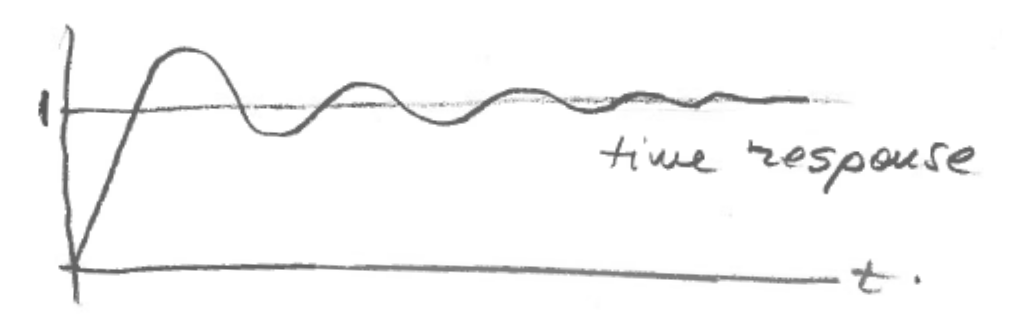
\includegraphics[width=3.5in]{../figures/x_t_time_response_2nd_order_step}
\end{figure}

\begin{mdframed}[middlelinewidth=0.5mm]
	\begin{center}
		\gr{Proof}
	\end{center}

\begin{figure}[H]
	\centering
	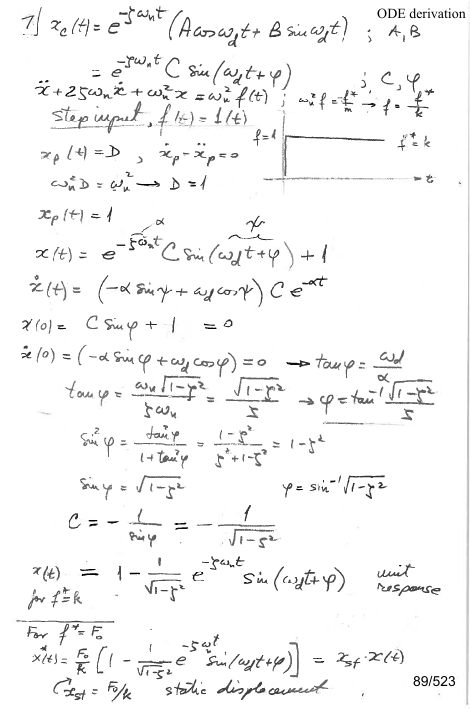
\includegraphics[width=5.5in]{../figures/x_t_time_response_2nd_order_step_proof_1}
\end{figure}
\begin{figure}[H]
	\centering
	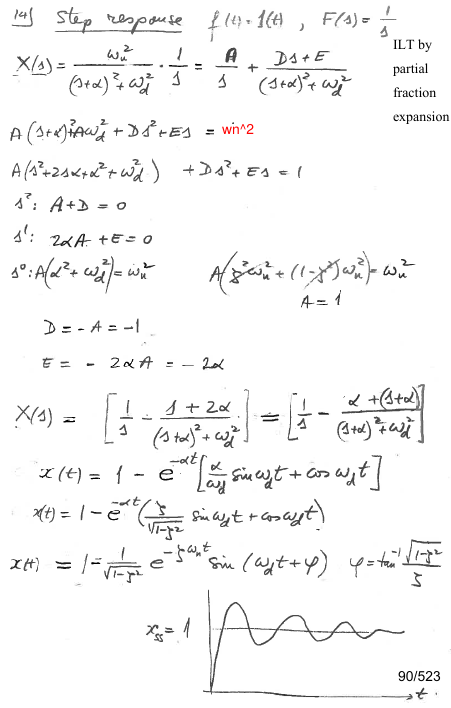
\includegraphics[width=5.5in]{../figures/x_t_time_response_2nd_order_step_proof_2}
\end{figure}
\end{mdframed}

\subsubsection{Impulse response of a 2\textsuperscript{nd} Order System}


\begin{align}
X(s) &= G(s)F(s) \\
&= \frac{\omega_n^2}{s^2 + 2 \zeta \omega_n s + \omega_n^2} \cdot 1\nonumber \\
&=  \frac{\omega_n^2}{s^2 + 2 \zeta \omega_n s + \omega_n^2}
\end{align}
Therefore, solving for $\Laplace{X(s)}^{-1}$ yields
\begin{equation}
x(t) = \frac{\omega_n}{\sqrt{1-\zeta^2}} e^{-\zeta \omega_n^2} \sin(\omega_dt)
\end{equation}
or
\begin{figure}[H]
	\centering
	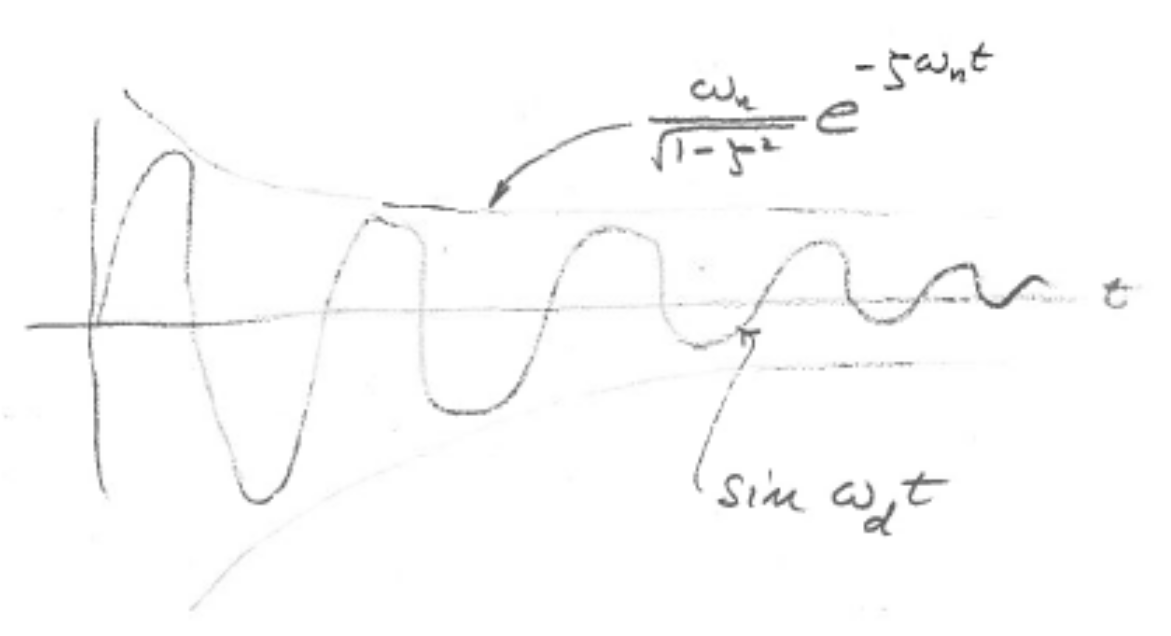
\includegraphics[width=4.5in]{../figures/x_t_impulse_time_response_2nd_order}
\end{figure}

\begin{mdframed}[middlelinewidth=0.5mm]
	\begin{center}
		\gr{Proof}
	\end{center}
	
	\begin{figure}[H]
		\centering
		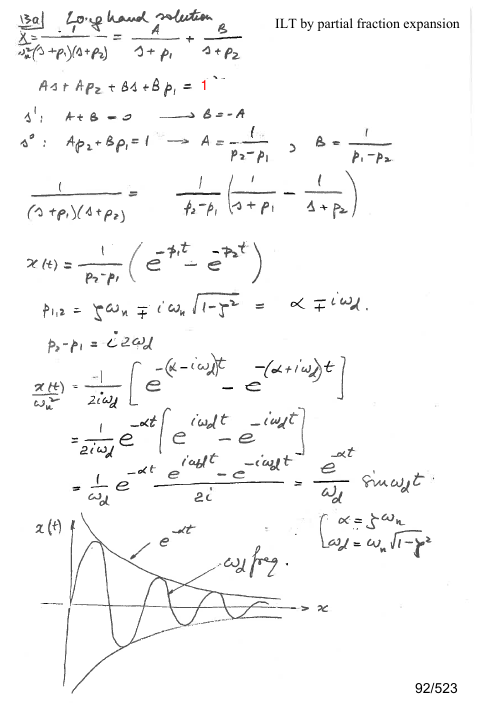
\includegraphics[width=5.5in]{../figures/x_t_time_response_2nd_order_impulse_proof_1}
	\end{figure}
	\begin{figure}[H]
		\centering
		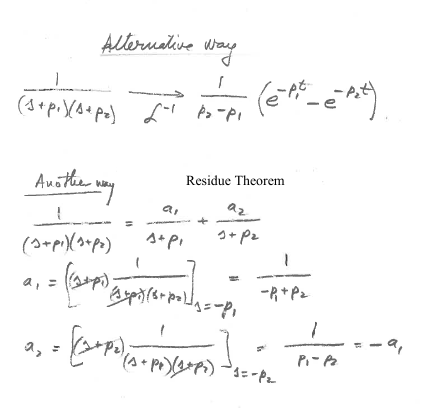
\includegraphics[width=5.5in]{../figures/x_t_time_response_2nd_order_impulse_proof_2}
	\end{figure}
\end{mdframed}

\subsubsection{Ramp response of a 2\textsuperscript{nd} Order System}


\begin{align}
X(s) &= G(s)F(s) \\
&= \frac{\omega_n^2}{s^2 + 2 \zeta \omega_n s + \omega_n^2} \cdot \frac{1}{s^2}\nonumber \\
&=  \frac{\omega_n^2}{s^2(s^2 + 2 \zeta \omega_n s + \omega_n^2)}
\end{align}
Therefore, solving for $\Laplace{X(s)}^{-1}$ yields
\begin{equation}
x(t) = t - \frac{2 \zeta}{\omega_n} \bigg( 1 + \frac{1}{\sin \gamma_1} e^{-\zeta \omega_n t}  \sin(\omega_dt - \gamma_1) \bigg)
\end{equation}
where
\begin{align}
\gamma_1 =& \tan^{-1} \frac{2 \zeta \sqrt{1-\zeta^2}}{1-2\zeta^2} \\
=& \sin^{-1} 2 \zeta \sqrt{1-\zeta^2}
\end{align}
or
\begin{figure}[H]
	\centering
	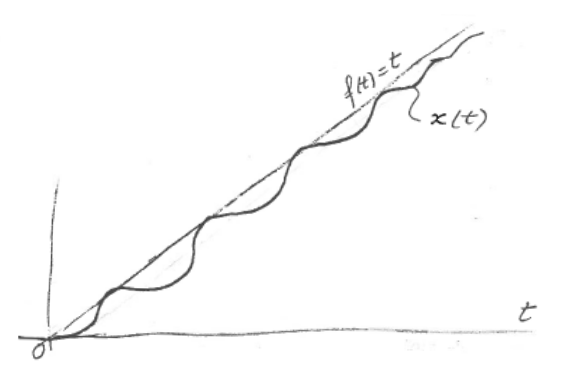
\includegraphics[width=3.5in]{../figures/x_t_ramp_time_response_2nd_order}
\end{figure}
Moreover, 
\begin{align}
\sin^2 \gamma_1 &= \frac{\tan^2 \gamma_1}{1 + \tan^2 \gamma_1}\\
 &= \frac{4 s^2 (1-\zeta^2)}{(1 - 2 \zeta^2)+ 4 \zeta^2(1-\zeta^2)} \nonumber \\
 &=  \frac{4 s^2 (1-\zeta^2)}{1-4s^2 + 4s^4 + 4s^2 - 4s^4} \nonumber \\
 &=  4 s^2 (1-\zeta^2) \nonumber
\end{align}
and
\begin{equation}
\sin \gamma_1 = 2 \zeta \sqrt{1-\zeta^2}
\end{equation}

\begin{mdframed}[middlelinewidth=0.5mm]
	\begin{center}
		\gr{Proof}
	\end{center}
	
	\begin{figure}[H]
		\centering
		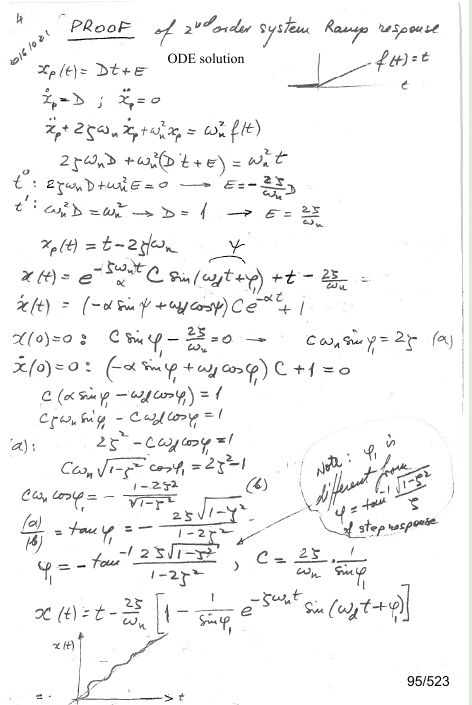
\includegraphics[width=5.5in]{../figures/x_t_time_response_2nd_order_ramp_proof_1}
	\end{figure}
\end{mdframed}

\subsubsection{Summary of the Second Order System Responses}

\begin{figure}[H]
	\centering
	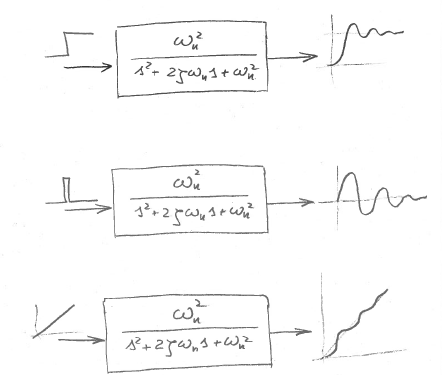
\includegraphics[width=4.5in]{../figures/Summary_of_second_order_system_response}
	\caption{A summary of the second order system responses.}
\end{figure}

\lstset{linewidth=5.8in}
\begin{minipage}{1\textwidth}
	\begin{center}
		\lstset{%
			caption={MATLAB code for time series responses of 2\textsuperscript{nd} order system.},
			basicstyle=\ttfamily\footnotesize\bfseries,
			frame=tb,
		}
		\begin{lstlisting}
%{
This program studies time response of 2nd order systems
%}

clc
clear
close all

format compact

%% Given data
fn = 5; % time response for the 1D system
wn = 2*pi()*fn
z = 0.035

%% time range setup
T_max = 10;         % run the test to 10 seconds
dt = T_max*1e-4;    % find the delta-t value 
t = 0:dt:T_max;     % build the time vector

%% Define system
B = [wn^2];
A = [1 2*z*wn wn^2];
G = tf(B,A); 

%% create the figure enviorment
figure(1)
xlim([0 1])

%% step response 
subplot(3,1,1)
hold on
step(G,t)
ylim([0 2])

%% Impulse response
subplot(3,1,2)
impulse(G,t)
ylim([-35 35])

%% Ramp response
F_ramp = tf([1],[1 0 0])
subplot(3,1,3)
impulse(G*F_ramp,t)
xlim([0 1])
ylim([0 1])
title('Ramp Response') % need to set manually. 
		\end{lstlisting}
	\end{center}
\end{minipage}

%
%\begin{example}
%	SIMULINK Tutorial 2\textsuperscript{nd} Order Systems 
%\end{example}

\subsection{Stability of response}


A system is stable if any stable input excitation produces a stable output response. 

\begin{figure}[H]
	\centering
	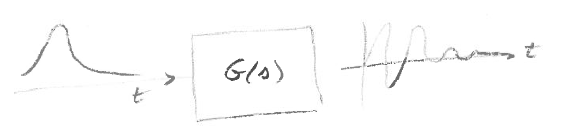
\includegraphics[width=5.5in]{../figures/stable_system_block_diagram}
\end{figure}

A response is stable if it remains bounded at $t \rightarrow \infty$

	\begin{figure}[H]
	\centering
	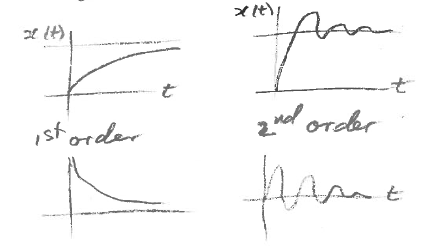
\includegraphics[width=4.5in]{../figures/stable_responses}
\end{figure}

\subsubsection{Stability of 1\textsuperscript{st}-Order Responses}

\begin{equation}
X(s) = \frac{K}{s-p}
\end{equation}

\begin{equation}
x(t) = K e ^{p t}
\end{equation}
where $p$ is the pole of $X(s)$. 

The stability is dictated by the sign of $p$, i.e. its location in the complex $p$-plane. If $P<0$ (or $p$ is in the left-hand-side), the system is stable. Therefore, if a disturbing force is applied, the system will return to its initial state.  


\begin{figure}[H]
	\centering
	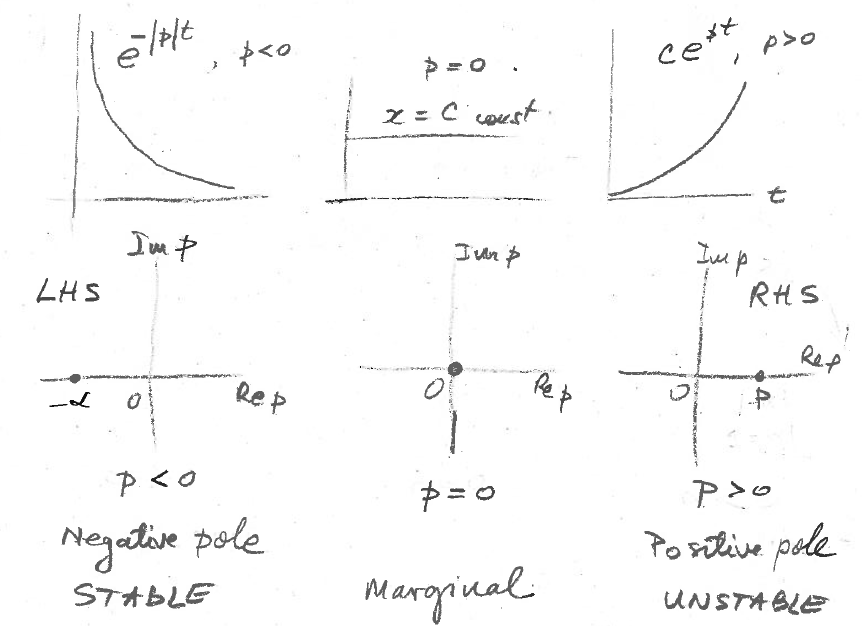
\includegraphics[width=4.5in]{../figures/system_stability_first_order}
\end{figure}

\subsubsection{Stability of 2\textsuperscript{nd}-Order Responses}

\begin{equation}
X(s) = \frac{k(s-z_1)}{(s-p_1)(s-p_2)}
\end{equation}

\begin{figure}[H]
	\centering
	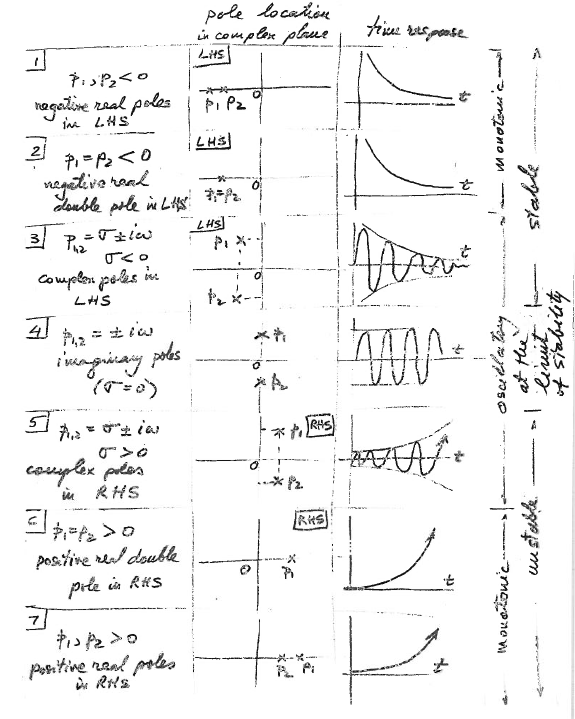
\includegraphics[width=4.5in]{../figures/2nd_order_poles}
\end{figure}

%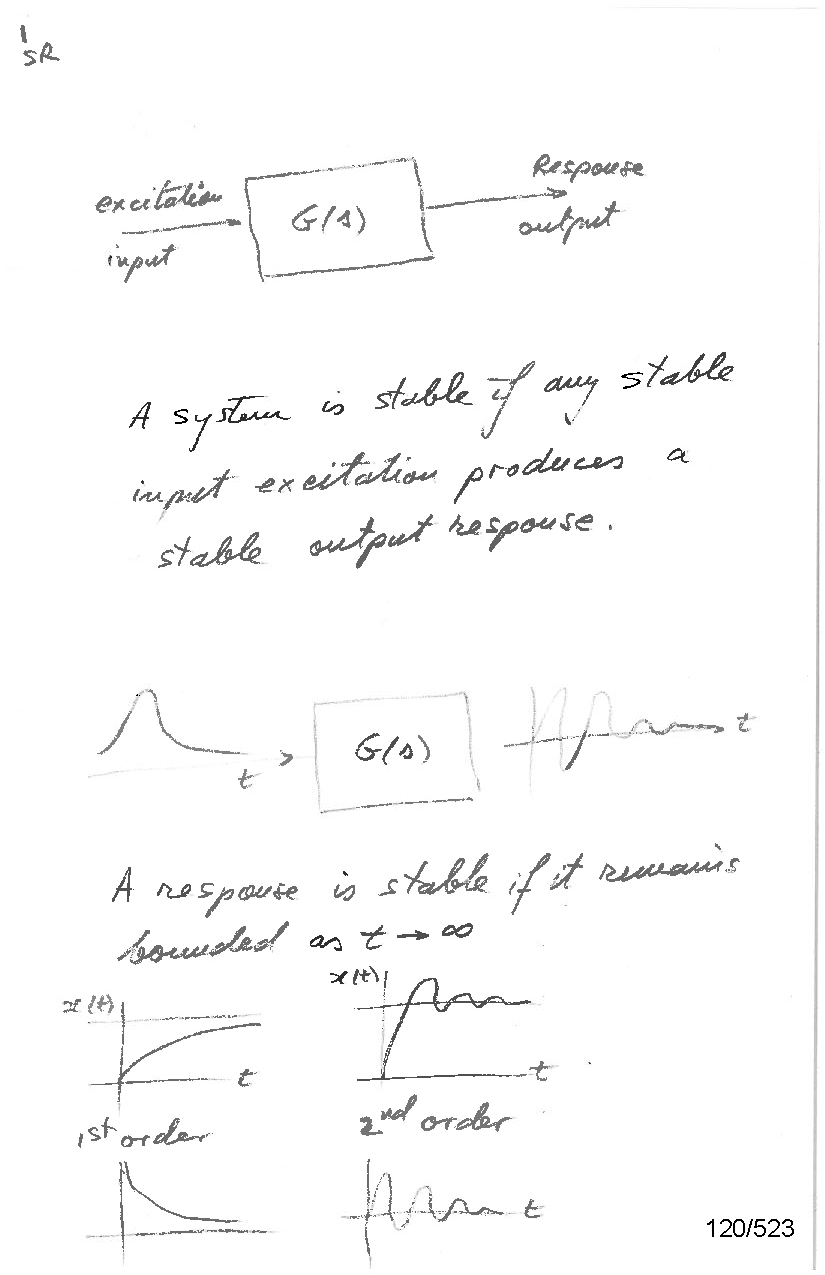
\includepdf[pages=-,pagecommand={},width=0.9\textwidth]{PDF_notes/Stability_of_response.pdf}


\subsubsection{Stability of Higher-order Responses}

Starting with a general expression for the output of a system
\begin{equation}
X(s) = \frac{B(s)}{A(s)} = \frac{b_ms^m+b_{m-1}s^{m-1} + \cdots + b_0}{a_ns^n+a_{n-1}s^{n-1} + \cdots + a_0}
\end{equation}
partial fraction expansion results in
\begin{equation}
X(s) = \frac{r_1}{s-p_1} + \frac{r_2}{s-p_2} + \cdots + \frac{r_n}{s-p_n}
\end{equation}
where $p_1, \; p_2, \; \cdots \; p_n$ are the poles of the system (i.e. roots of $A(s)=0$) and $r_1,\; r_2,\; \cdots \; r_n$ are the residues of the system. Note that the poles can either be real or complex. Again, MATLAB can be used to solve for the roots, poles, and gains of the system using \texttt{[r,p,k]=residue(B,A)}. The real poles can be
\begin{itemize}
	\item single pole: $\frac{r}{s-p} \xrightarrow{\Laplace{\; \; \;}^{-1}} re^{pt}$
	\item double poles: $\frac{r}{(s-p)^2} \xrightarrow{\Laplace{\; \; \;}^{-1}} rte^{pt}$
	\item multiple poles: $\frac{r}{(s-p)j} \xrightarrow{\Laplace{\; \; \;}^{-1}} \frac{1}{(j-1)!}t^{j-1}e^{pt}$
\end{itemize} 
where stable and unstable responses are
\begin{figure}[H]
	\centering
	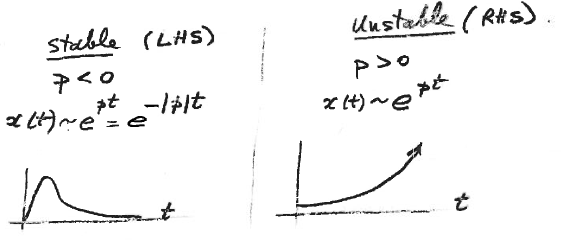
\includegraphics[width=4.5in]{../figures/stability_higher_order_systems_real_poles}
\end{figure}
The complex poles are always in conjugate pairs, and are governed by $p_{1,2}=\sigma \pm i \omega$ where
\begin{itemize}
	\item first pole: $\frac{1}{s-p_1} = \frac{1}{s-(\sigma + i \omega)} \xrightarrow{\Laplace{\; \; \;}^{-1}} e^{(\sigma + i \omega)t} = e^{\sigma t} e^{i \omega t}$
	\item second pole: $\frac{1}{s-p_2} = \frac{1}{s-(\sigma - i \omega)} \xrightarrow{\Laplace{\; \; \;}^{-1}} e^{(\sigma - i \omega)t} = e^{\sigma t} e^{-i \omega t}$
\end{itemize} 
Using Euler's formula, this results in
\begin{equation}
x(t) = e^{\sigma t} (e^{i \omega t}-e^{-i \omega t}) = e^{\sigma t} \sin(\omega t) 
\end{equation}
where stable and unstable responses are
\begin{figure}[H]
	\centering
	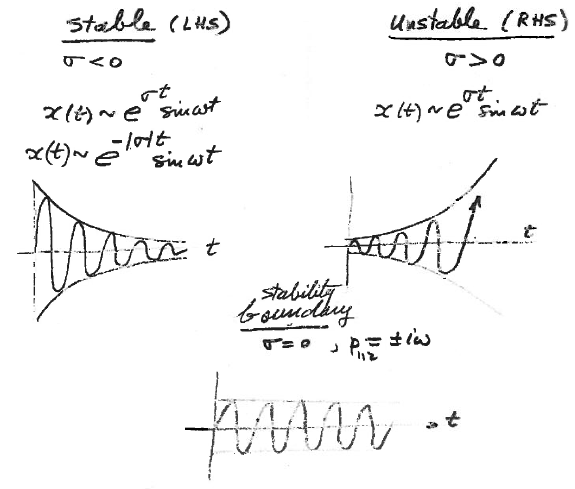
\includegraphics[width=4.5in]{../figures/stability_higher_order_systems_complex_poles}
\end{figure}

\subsubsection{Absolute Stability}
A necessary and sufficient condition for a system to be stable is that its poles are placed in the Left hand side of the complex plane. 
\begin{figure}[H]
	\centering
	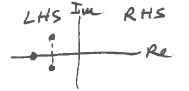
\includegraphics[width=2.5in]{../figures/stable_system_complex_plane_simple}
\end{figure}

\subsubsection{Marginal Stability}
If the poles are purely imaginary (i.e. placed on the imaginary axis) then the system as marginal stability. 
\begin{itemize}
	\item bounded impulse response, the system is stable
	\item unbounded impulse response, or other inputs, the system is not stable. 
\end{itemize}

\subsubsection{Relative Stability}
Would a stable system still be stable if its parameters are slightly changed? What margin of safety is there?






	\pagebreak
	\renewcommand{\thepage}{}
	\renewcommand\refname{References Cited}
	\pagestyle{plain}
	\bibliographystyle{Downey_NSF}
	\bibliography{Chapter_1_Basic_Concepts}


















\end{document}

